\chapter{Modules}
\label{hoofdstuk:modules}
In dit hoofdstuk komen de voor dit thesisproject ontwikkelde modules aan bod. Zij proberen elk de collectie paarvoorstellen op een andere manier voor te stellen om een beter overzicht te cre\"eren of sneller individuele paren te beoordelen.\\

Modules kunnen ervoor kiezen het model dat ze toegewezen krijgen te manipuleren of niet. Indien wel, zullen alle modules die dit model delen steeds de veranderingen volgen.

\section{MatchTileView}

\begin{figure}[!h]
	\begin{center}
		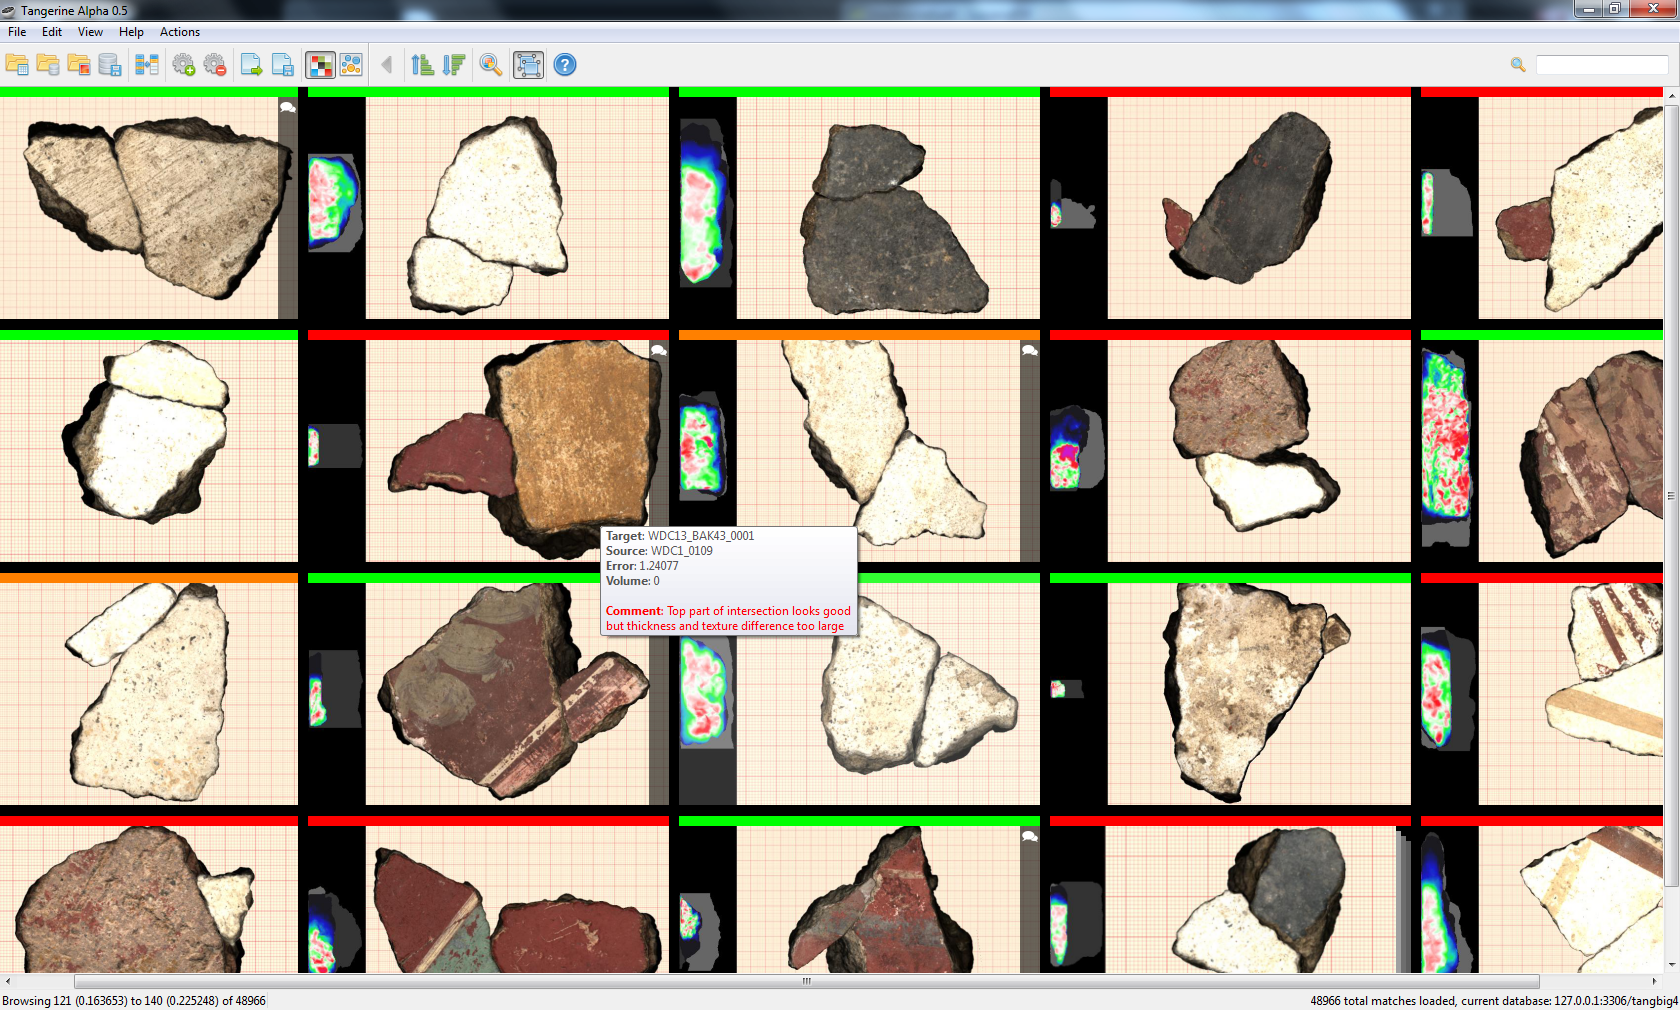
\includegraphics[width=1.0\columnwidth]{images/matchtileview-nice-01.png}
		\caption{De \emph{MachTileView}-module}
		\label{fig:mtv1}
	\end{center}
\end{figure}

\emph{MatchTileView} is de meest uitgewerkte module en stelt de gebruiker in staat om op effici\"ente wijze te zoeken naar de gewenste paren. De manier waarop het die weergeeft is gebaseerd op Browsematches: een dambordpatroon van paren met aan de linkerkant de doorsnede van hun raakvlak en vanboven een kleurcode die aangeeft wat de huidige validatie is\footnote{Groen: zeker correct, Oranje: misschien correct, Rood: zeker niet correct, Grijs: in conflict, Zwart: niet gekend}. De doorsnede is roder/paarser op plaatsen waar de volumes van de fragmenten dieper in elkaar snijden, wit waar ze op elkaar passen en blauwer hoe verder ze uit elkaar staan. Uit ervaring blijkt dat de doorsnede relevant is om te beslissen of een paar interessant is~\cite{Brown2010}. Als men in de realiteit fragmenten op elkaar past, is het natuurlijk niet mogelijk om de doorsnede te bekijken, met als gevolg dat dit nuttige perspectief alleen virtueel te verkrijgen valt. Om deze reden kan de module optioneel enkel de doorsnedes weergeven, waardoor er veel meer paren op een scherm passen (zie figuur~\ref{fig:tileview-reduced-compare}). De aanwezigheid van bepaalde attributen, zoals commentaren of duplicaten, worden visueel weergegeven met iconen en andere tekenstijlen.\\

Met de pijltoetsen kunnen gebruikers navigeren in de verzameling, de statusbalk geeft steeds weer op het hoeveelste scherm men zit en hoeveel paren er aan de huidige criteria voldoen. Er is een werkbalk waarin gebruikers kunnen kiezen op welke eigenschappen er gesorteerd en gefilterd moet worden. Sommige operaties zoals duplicaten uitzetten en verschillende validaties weergeven worden zo frequent toegepast dat ze een eigen knop krijgen op de werkbalk.\\

\begin{figure}[ht]
	\begin{center}
		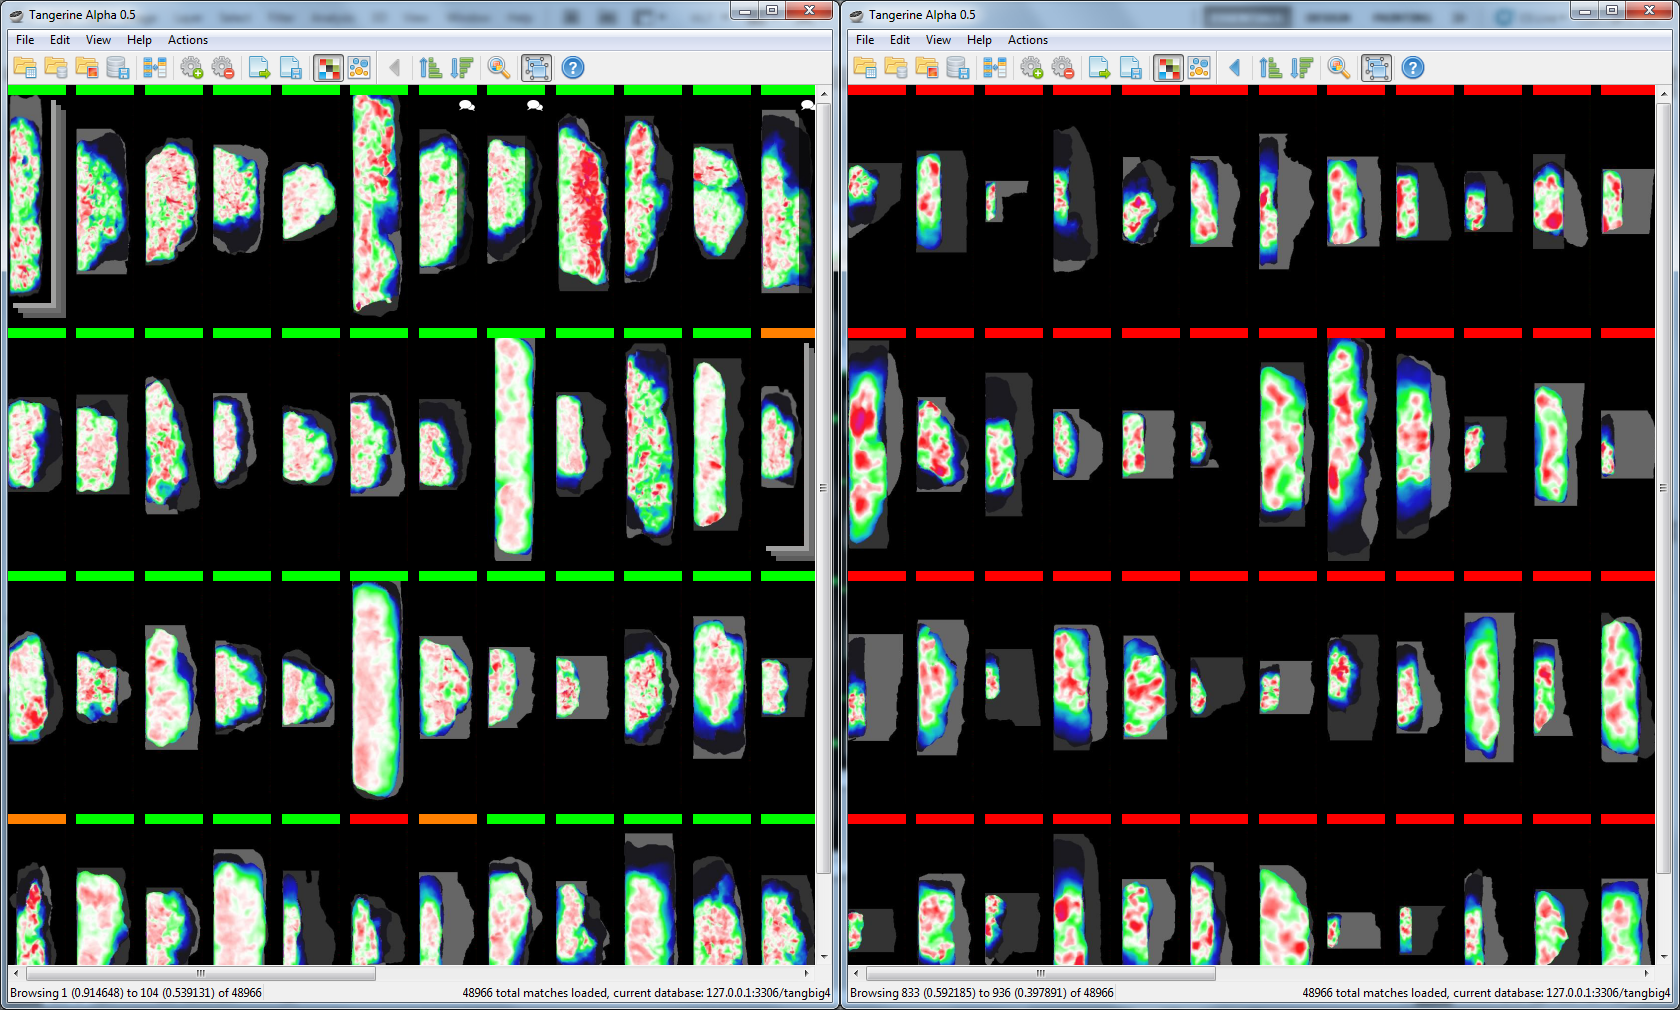
\includegraphics[width=1.0\columnwidth]{images/tileview-reduced-compare-01.png}
		\caption{De doorsnedes van goede paren tegenover die van slechte paren. Een mens kan met ervaring leren om hieruit reeds veel af te leiden. Yassine Ryad bewees dat een algoritme kan gemaakt worden dat deze informatie in een rangschikking omzet.~\cite{Ryad2011}}
		\label{fig:tileview-reduced-compare}
	\end{center}
\end{figure}

In het rechterklikmenu bevinden zich een aantal geavanceerdere filtermogelijkheden die van toepassing zijn op een paar: 

\begin{packed_itemize}
  \item vind alle buren van het paar
  \item vind alle buren van het paar die ermee conflicteren
  \item vind alle buren van het paar die er niet mee conflicteren
  \item vind alle buren van het paar die er niet mee conflicteren en ook niet met elkaar conflicteren
\end{packed_itemize}

Een conflict komt voor als een deel van de rand van een fragment door twee verschillende fragmenten ingenomen wordt. Het kan best zijn dat twee fragmenten niet op dezelfde plaats aansluiten op een andere fragment, maar wel onderlinge volumeintersecties hebben. Dit soort conflicten ook in acht nemen is een toekomstige onderzoeksrichting. De voornoemde operaties zijn vooral handig op voorstellen die reeds te boek staan als \emph{correct} (of zelfs \emph{misschien correct}). De conflicterende buren kunnen bijvoorbeeld onmiddellijk verworpen worden. Tussen de buren die niet conflicteren kan mogelijk een interessant paar zitten. \\

De laatste optie stelt een cluster rond het geselecteerde paar op. Het proces gaat als volgt: de database wordt gevraagd naar alle buren van het huidige paar, gerangschikt op een maatstaf naar keuze zoals de \emph{fout} of de \emph{probabiliteit}. Elke buur wordt dan op het orignele paar geplaatst als de plaats waar die zou terechtkomen nog vrij is. Eerst worden de \emph{correct}-verbindingen aan de cluster toegevoegd, dan de \emph{misschien}-verbindingen, enzoverder. Binnen een validatie wordt er toegevoegd in de volgorde van de maatstaf. Figuur~\ref{fig:tileview-progconflict} laat het resultaat van deze operatie op het linksbovenste voorstel zien. In sectie~\ref{sec:detailview} wordt de module besproken die het aan elkaar gepuzzelde resultaat kan weergeven. \\

\begin{figure}[ht]
	\begin{center}
		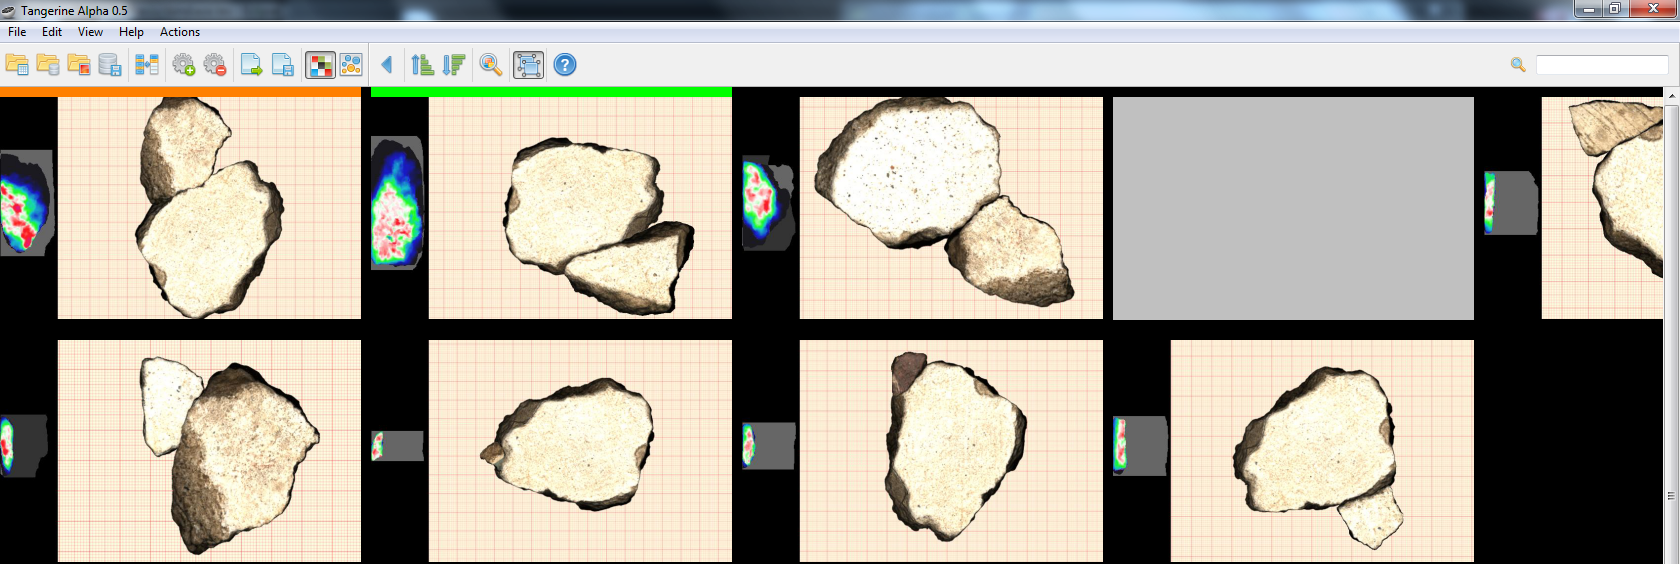
\includegraphics[width=1.0\columnwidth]{images/matchtileview-progconflict-01-reduced.png}
		\caption{Paren die niet conflicteren met elkaar}
		\label{fig:tileview-progconflict}
	\end{center}
\end{figure}

\emph{MatchTileView} kan niet enkel gebruikt worden om te bekijken, maar ook om attributen te veranderen. Men kan onder andere commentaren toevoegen en validaties veranderen. Aanduiden dat bepaalde paren duplicaten zijn gaat ook, hoewel het gemakkelijker is dit door een algoritme te laten bepalen.\\

Als laatste is er kopieerfunctionaliteit, met de gebruikelijke sneltoetsen of het rechterklikmenu kunnen paren naar Griphos overgezet worden om ze in meer detail te bekijken.

\section{DetailView}
\label{sec:detailview}

\emph{DetailView} is een hulpmodule die door andere modules gebruikt wordt om weer te geven wat er kan bij elkaar gepuzzeld worden. Dit is gelijkaardig aan het tafelblad van Griphos, met het verschil dat men met \emph{DetailView} vrij kan navigeren in een 3D-wereld. Hun opzet is verschillend: met Griphos kan manueel gepuzzeld worden, terwijl \emph{DetailView} dient om automatische reconstructies te beoordelen. Dubbelklikken op alle voorstellen in figuur~\ref{fig:tileview-progconflict} zal deze aan elkaar zetten en weergeven in \emph{DetailView}. Het resultaat is figuur~\ref{fig:detailfull}.\\

\begin{figure}[ht]
	\begin{center}
		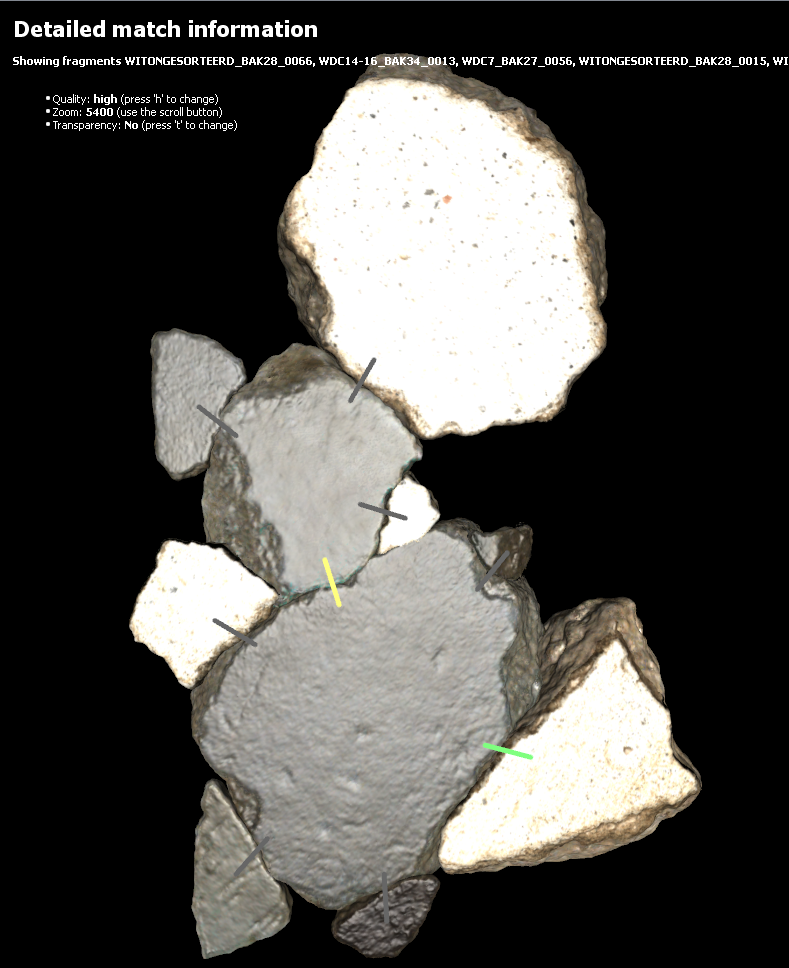
\includegraphics[width=1.0\columnwidth]{images/detailview-interesting-thin.png}
		\caption{\emph{DetailView}: De paren van figuur~\ref{fig:tileview-progconflict} aan elkaar gemaakt in 3D}
		\label{fig:detailfull}
	\end{center}
\end{figure}

\FloatBarrier

\begin{figure}[!hbt]
  \centering
  %\subfloat[De cluster]{\label{fig:detailfull}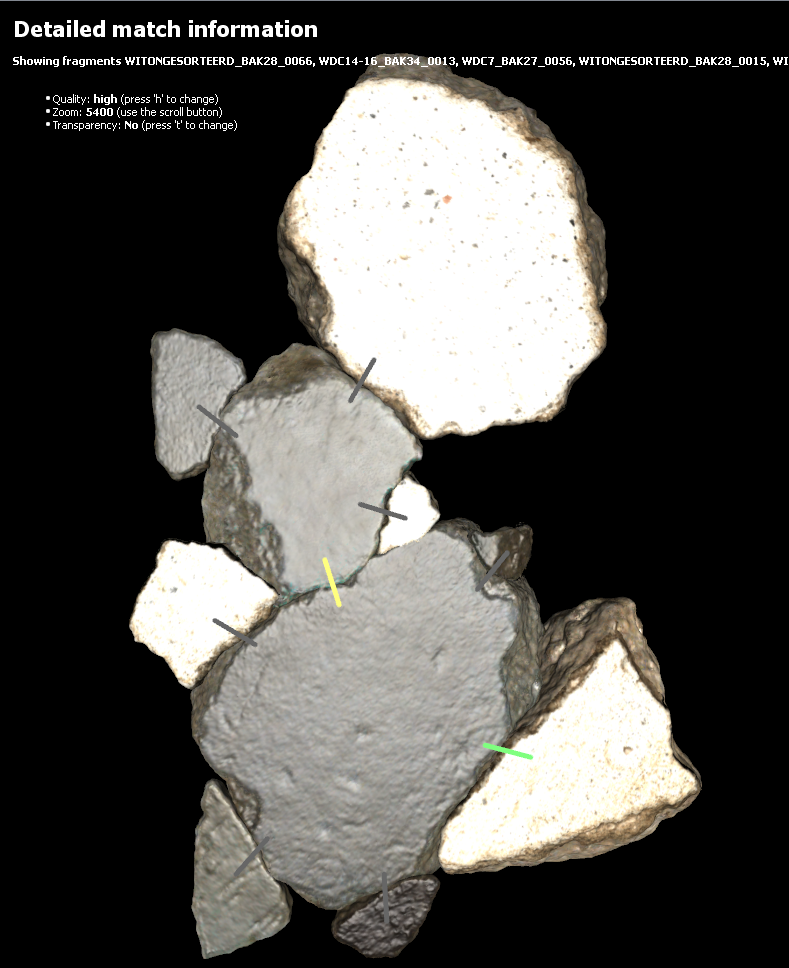
\includegraphics[width=0.33\textwidth]{images/detailview-interesting-thin.png}}                
  \subfloat[Een betere kijk op het interessante stuk]{\label{fig:detailzoom}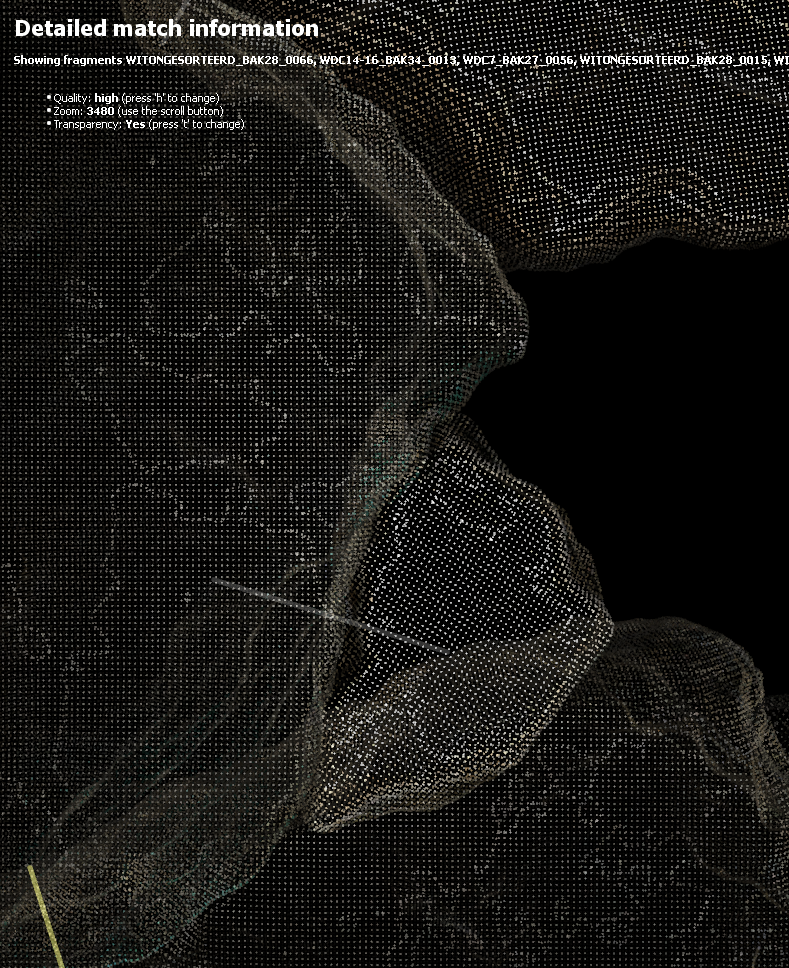
\includegraphics[width=0.47\textwidth]{images/detailview-interesting-thin-zoom.png}}
  \subfloat[De achterkant van het interessante stuk]{\label{fig:detailreverse}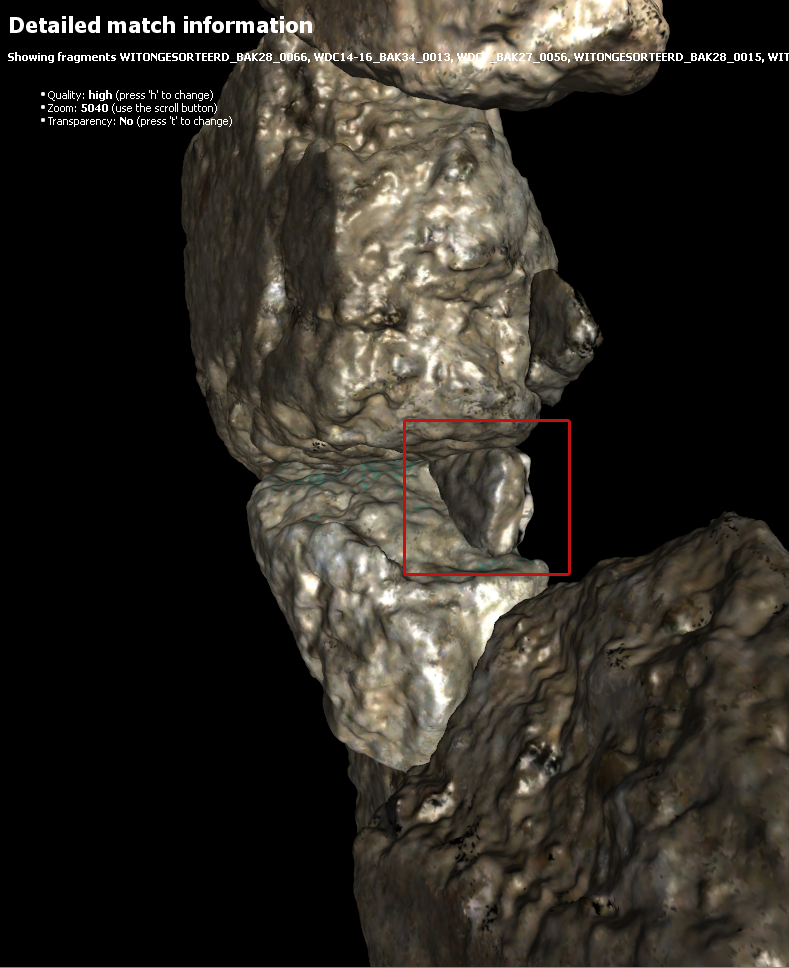
\includegraphics[width=0.47\textwidth]{images/detailview-interesting-thin-zoom-reverse-2.png}}
  \caption{\emph{DetailView} kan gebruikt worden om paren vanuit verschillende standpunten te bekijken}
  \label{fig:detail1}
\end{figure}

Figuur~\ref{fig:detailfull} is informatiever dan het dambordpatroon van \emph{MatchTileView} omdat het nuttige contextinformatie geeft. Het komt vaak voor dat door erosie een voorstel plausibel lijkt maar toch verkeerd is, maar het is veel minder waarschijnlijk dat drie fragmenten plausibel in elkaar passen en verkeerd zijn. Het kleine witte fragment dat geklemd zit tussen de twee grote grijze brokken is hier een voorbeeld van. Merk op dat de kleur van de fragmenten in dit specifieke voorbeeld niet zo relevant is\footnote{door vari\"erende brokstukkwaliteit en scancondities kunnen zelfs in een correct paar grote kleurverschillen optreden}, dit valt ook te merken in het grote kleurverschil bij het reeds goedgekeurde paar.\\

In eerste aanleg lijkt het er op dat een voorheen ongekende connectie is ontdekt, maar een dichtere inspectie toont een paar problemen. Figuur~\ref{fig:detailzoom} toont het geklemde fragment van dichterbij en geeft de geometrie weer als een puntenwolk, waardoor intersecties zichtbaar worden. Spijtig genoeg lijkt het erop dat een aanzienlijk volume van het geklemde fragment in het onderste grijze brokstuk zit\footnote{Dit is minder duidelijk op een kleine afbeelding maar goed te zien op een computerscherm, zeker als er tussen weergaven gewisseld wordt.}. De grafische voorstelling roteren onthult dat het geklemde fragment ook veel dunner is dan de rest, wat weer een aanwijzing is dat het misschien geen goed paar is. Desalniettemin zou dit best eens nagekeken worden met de echte brokstukken.

\section{GraphView}
Pure grafische plugins kunnen vertrouwen op andere plugins voor data-selectie: Om de werkbaarheid van dit systeem uit te testen werd een voorbeeldmodule ontwikkeld die alle huidige paren op een graaf plaatst en hier een ontwarringsalgoritme op toepast met behulp van de GraphViz bibliotheek. Deze voorstelling geeft een globaler beeld van de paren die aan de geldende criteria van het model voldoen.\\

Een gebruiksscenario is bijvoorbeeld om in \emph{MatchTileView} alle paren op te vragen die \emph{correct} of \emph{misschien correct} zijn, en daarna over te schakelen naar \emph{GraphView}. Dit werd gedaan op een database van 50000 paren, de criteria lieten er 245 over. Figuur~\ref{fig:graphyesmaybe} is het resultaat.\\

\begin{figure}[ht]
	\begin{center}
		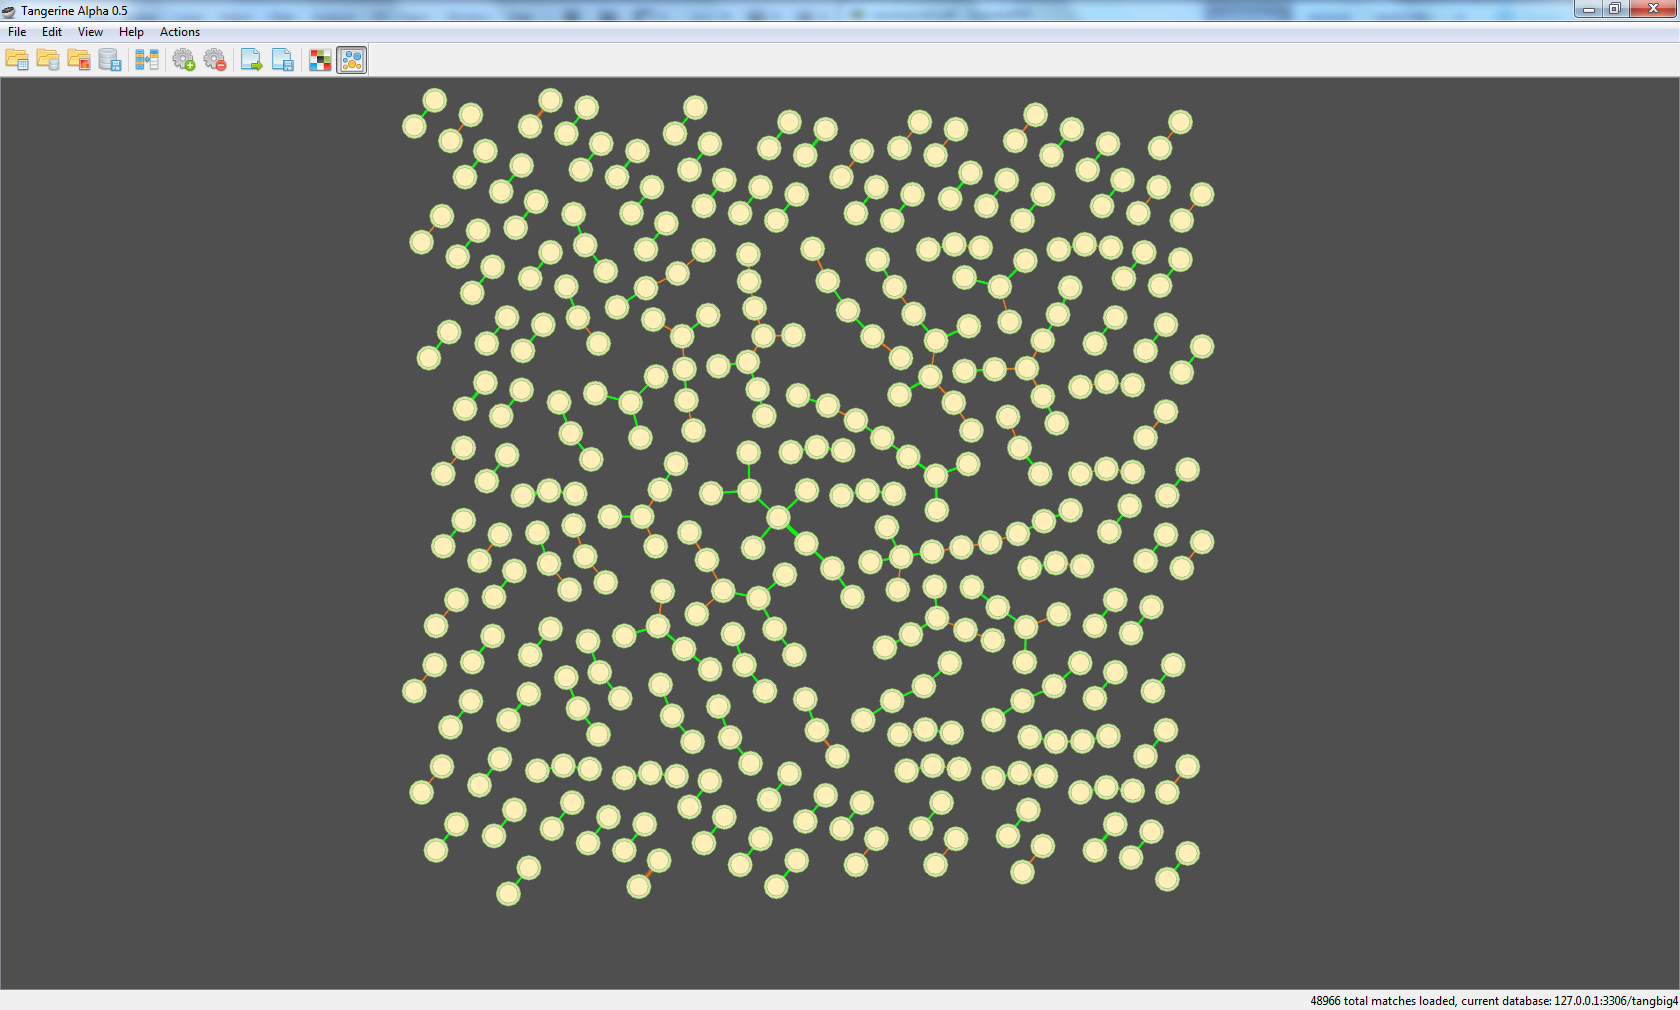
\includegraphics[width=1.0\columnwidth]{images/nodeview-yesmaybe.png}
		\caption{\emph{GraphView}: alle \emph{correcte} en \emph{misschien correcte} paren als een graaf voorgesteld}
		\label{fig:graphyesmaybe}
	\end{center}
\end{figure}

Hoe meer fragmenten er in een ketting aan elkaar kunnen gemaakt worden, hoe meer naar het midden ze worden gezet door het ontwarringsalgoritme. Nu de kettingen gemakkelijk zichtbaar zijn kunnen ze ook gevisualiseerd worden in 3D zoals in figuren~\ref{fig:graphchain1} en~\ref{fig:graphchain2}. Het valt op dat uit beide figuren gemakkelijk af te leiden valt welke \emph{misschien correcte} paren zeker niet correct zijn door naar de volumeoverlappingen te kijken (in~\ref{fig:graphchain1} zitten er zelfs een paar fragmenten volledig in een ander fragment).

\begin{figure}[ht]
	\begin{center}
		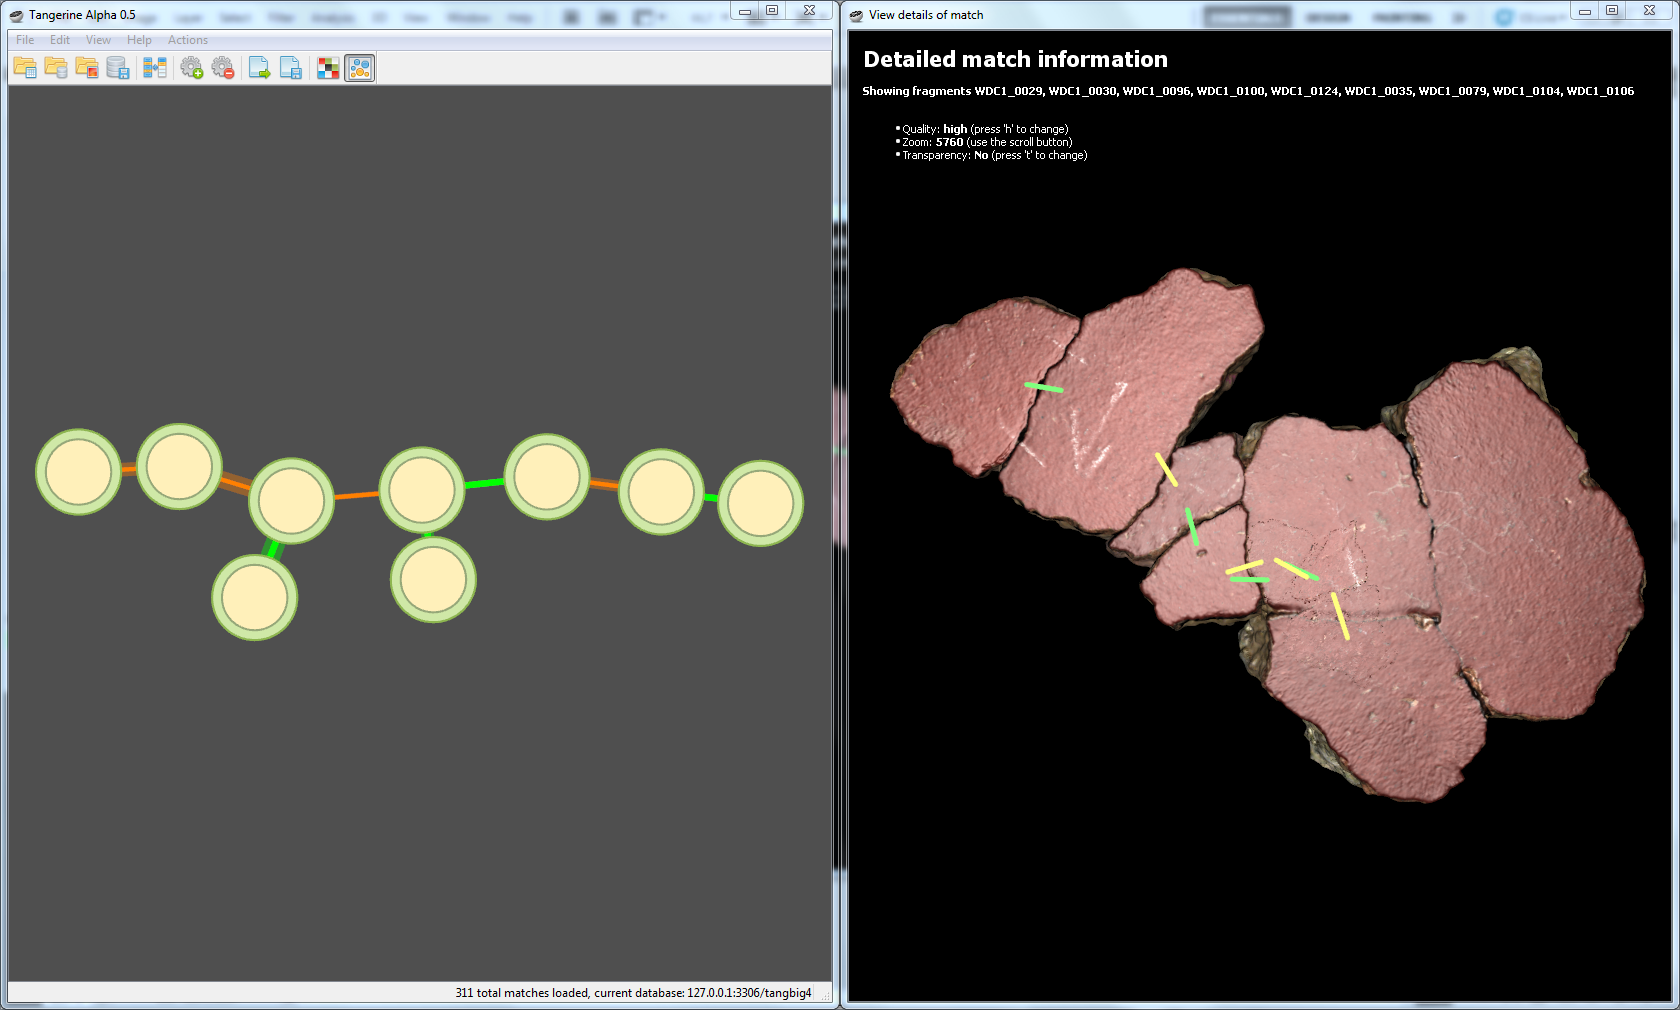
\includegraphics[width=1.0\columnwidth]{images/detailview-chain-02-rawcut.png}
		\caption{\emph{GraphView}: een ketting voorstellen in 3D}
		\label{fig:graphchain1}
	\end{center}
\end{figure}

\begin{figure}[ht]
	\begin{center}
		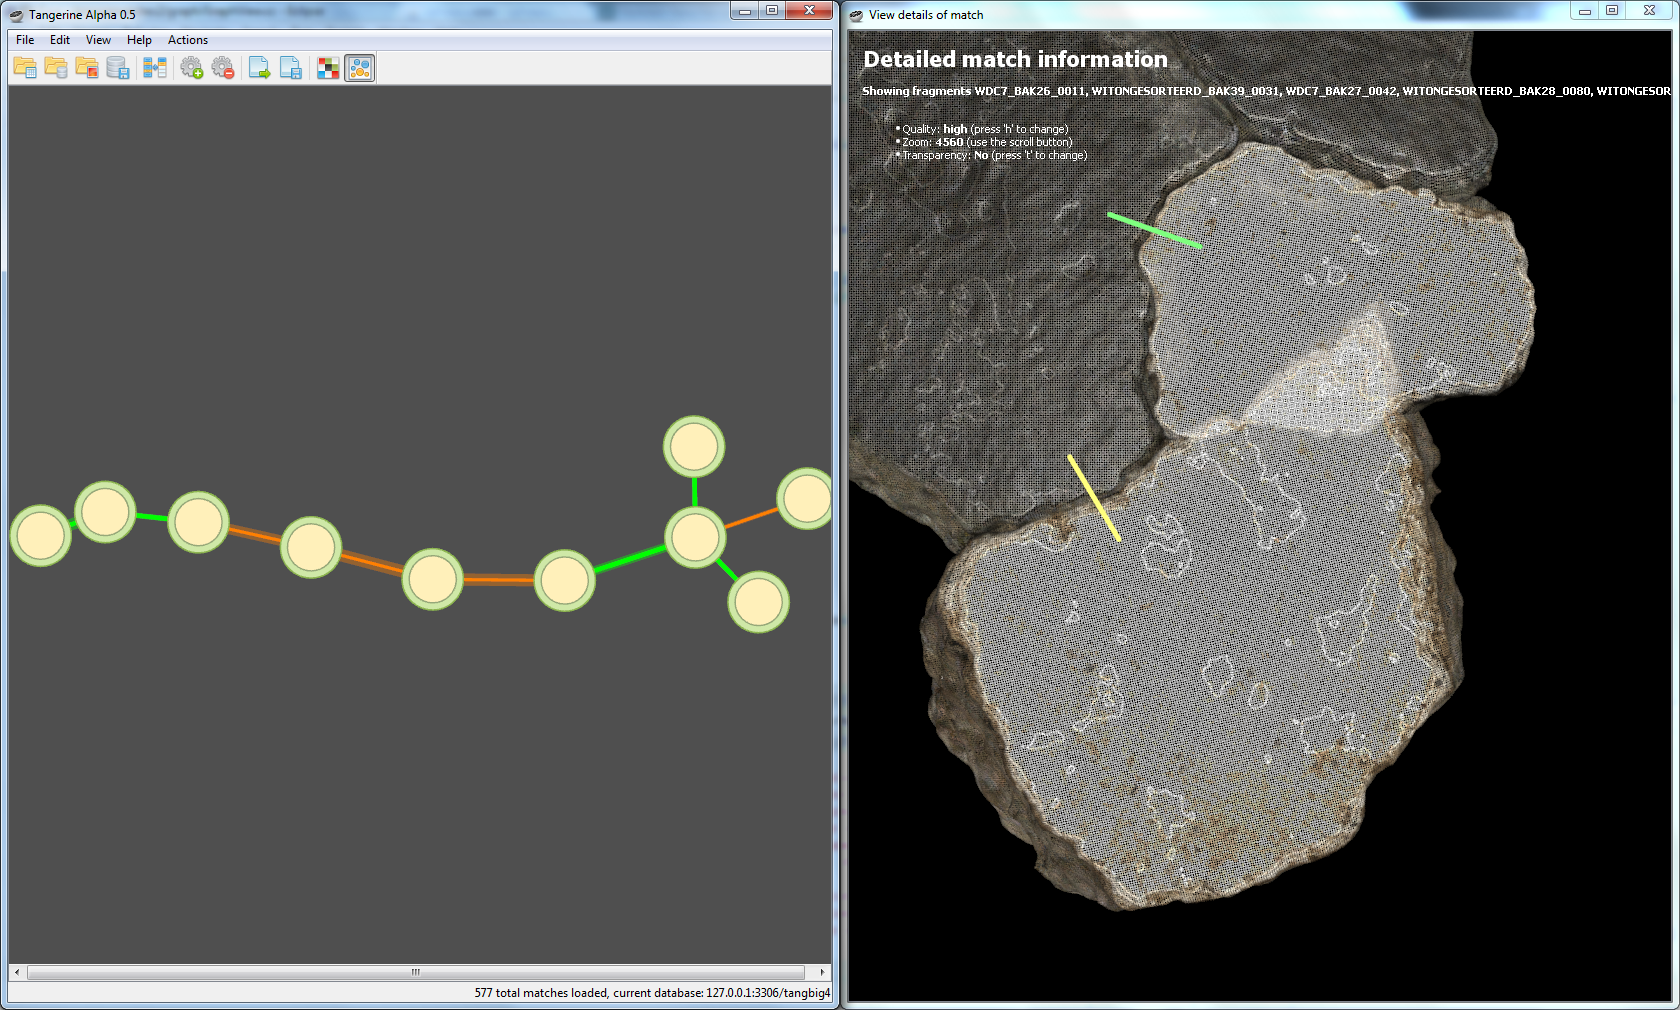
\includegraphics[width=1.0\columnwidth]{images/detailview-chain-10-rawcut.png}
		\caption{\emph{GraphView}: een andere ketting voorstellen in 3D}
		\label{fig:graphchain2}
	\end{center}
\end{figure}